\documentclass[border=10pt]{standalone}
\usepackage{pgfplots}
\pgfplotsset{compat=1.17}
\begin{document}
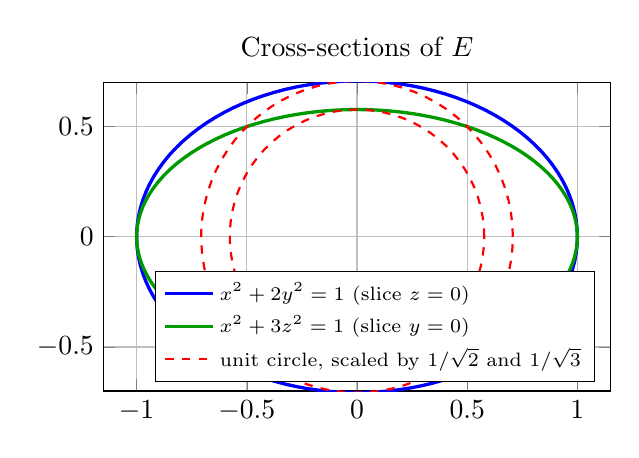
\begin{tikzpicture}
\begin{axis}[
    width=11cm, height=5.5cm,
    xlabel={}, ylabel={},
    title={Cross-sections of $E$},
    xmin=-1.15, xmax=1.15, ymin=-0.7, ymax=0.7,
    axis equal image,
    grid=major,
    legend pos=south east,
    legend cell align=left,
    legend style={font=\scriptsize},
]
% z = 0 slice: x^2 + 2y^2 = 1
\addplot[blue, very thick, domain=0:360, samples=120]
    ({cos(x)}, {sin(x)/sqrt(2)});
\addlegendentry{$x^2+2y^2=1$ (slice $z=0$)}
% y = 0 slice: x^2 + 3z^2 = 1
\addplot[green!60!black, very thick, domain=0:360, samples=120]
    ({cos(x)}, {sin(x)/sqrt(3)});
\addlegendentry{$x^2+3z^2=1$ (slice $y=0$)}
% scaled unit circles
\addplot[red, dashed, thick, domain=0:360, samples=80]
    ({cos(x)/sqrt(2)}, {sin(x)/sqrt(2)});
\addplot[red, dashed, thick, domain=0:360, samples=80]
    ({cos(x)/sqrt(3)}, {sin(x)/sqrt(3)});
\addlegendentry{unit circle, scaled by $1/\sqrt{2}$ and $1/\sqrt{3}$}
\end{axis}
\end{tikzpicture}
\end{document}